\chapter{Preliminaries and Foundations}
\label{ch:preliminaries}

This chapter is logically divided into two main parts. The first part presents the tooling and techniques I utilized to implement the space-reduction solution. The first section \ref{sec:notation} introduces common notations and terminologies used through out the work. Next, the pointer tagging technique is presented in section \ref{sec:preliminaries:pointertagging}. \\ 

In the second part, the the semantic web topic is visited in section \ref{sec:preliminaries:semanticweb}) before delving into into Tentris in section \ref{sec:preliminaries:tentris} where its concept and implementation are discussed. 

\section{Notation and Convention}
\label{sec:notation}

For a function $f$, the domain and co-domain of $f$ are denoted by dom($f$) and codom($f$), respectively. The set of natural numbers $\mathbb{N}$ includes zero in this work. Further $\mathbb{N}_{n}$ with $n \in \mathbb{N}$ is equal to $\{0, 1, ..., n -1\}$.
We use angle brackets $<...>$ to define a tuple $t$ which represents a sequence with fixed order for its elements. The entries $<t_0, t_1, ... , t_{n-1}>$ of a tuple $t$ with length $n$ can be accessed using the square bracket notation (subscript) after the tuple symbol. 
For example, $t[i]=t_i$ is the tuple $t$ entry at position $i$. 
Entries of a tuple $t$ are zero-indexed. 
The domain of a tuple $t$, denoted by dom($t$) = $<0,1,...,n-1>$, is a tuple of $t$ entries' positions.


\section{Pointer Tagging}
\label{sec:preliminaries:pointertagging}

Pointer Tagging \cite{taggedpointer} is a low-level programming technique that uses the spare low bits in a pointer to encode additional information. Using the Pointer tagging technique, pointer value (initially a memory address before tagging) can hold extra information, \textit{a tag}. The tag can hold extra information about the point-to heap object or can be used as meta-data to further describe the usage of the pointer data. Pointer tagging is mainly enabled because of the way heap objects are situated and accessed on modern computer architectures.

\subsection{Data Structure Alignment}
\label{sec:preliminaries:data_alignment}
Data alignment (also referred to as data structure padding) is a way in which heap objects are arranged and accessed by the CPU. CPUs in modern computer architecture (say 64-bit architecture) read data from and write data to memory more efficiently when data is aligned.  \\

On an abstract level, computer memory can be seen as an array of words or bytes, each with its own address. Unlike bytes, the term word has ambiguate meaning. In the context of this work, we are targeting the generic term in the context of CPU architecture. That is, a "processor word" refers to the size of a processor register or memory address register. The term word also refers to the size of CPU instruction, or the size of a pointer depending on the exact CPU architecture \cite{OSConcept}. For example, in a 64-bit architecture, the word size (also pointer size) is 64 bits = 8 bytes.\\

Generally, when a source program is executed, it is loaded into memory and put into a process $p$ for execution. All data objects in the program are mapped at certain point in time (during compilation or execution) to a physical memory address \cite{OSConcept}. Let us take, as an example, the following coding snippet written in C++:

\begin{verbatim}
bool *p1 = new bool(true);     // p1 = 0x011F0
int  *p2 = new int(123);       // p2 = 0x11608
char *p3 = new char(‘A’);      // p3 = 0x117A8
\end{verbatim}

The execution of the snippet will metaphorically results in a memory layout similar to the one presented in figure \ref{fig:data_aligntment}. According to C++ language specification \cite{cpp}, the size of integer value in memory is 4 bytes, the size of char is 1 byte, and short is 2 bytes. When we execute the previously mentioned statements, however, the compiler (or linker) books 8 bytes of memory to hold the integer value and not 4 bytes as expected. The reason is that, the compiler adds padding to the heap objects in order to align them in memory. The same applies to the character value (Fig. \ref{fig:data_aligntment}).  \\

Why data alignment? The CPU can access the memory only in word-sized chunks. So if our data always starts at a word it can be fetched efficiently. If data was to start somewhere in the middle of a word, the CPU will need to wait two or more memory cycles to fetch data from or write data to memory causing an increase in the CPU \textit{stall} period which results in a significant performance overhead  \cite{OSConcept}. \\


many modern compilers implementations handle data alignment in memory automatically, example includes C, C++, Rust, C\# compilers.

\begin{figure}
	\centering
	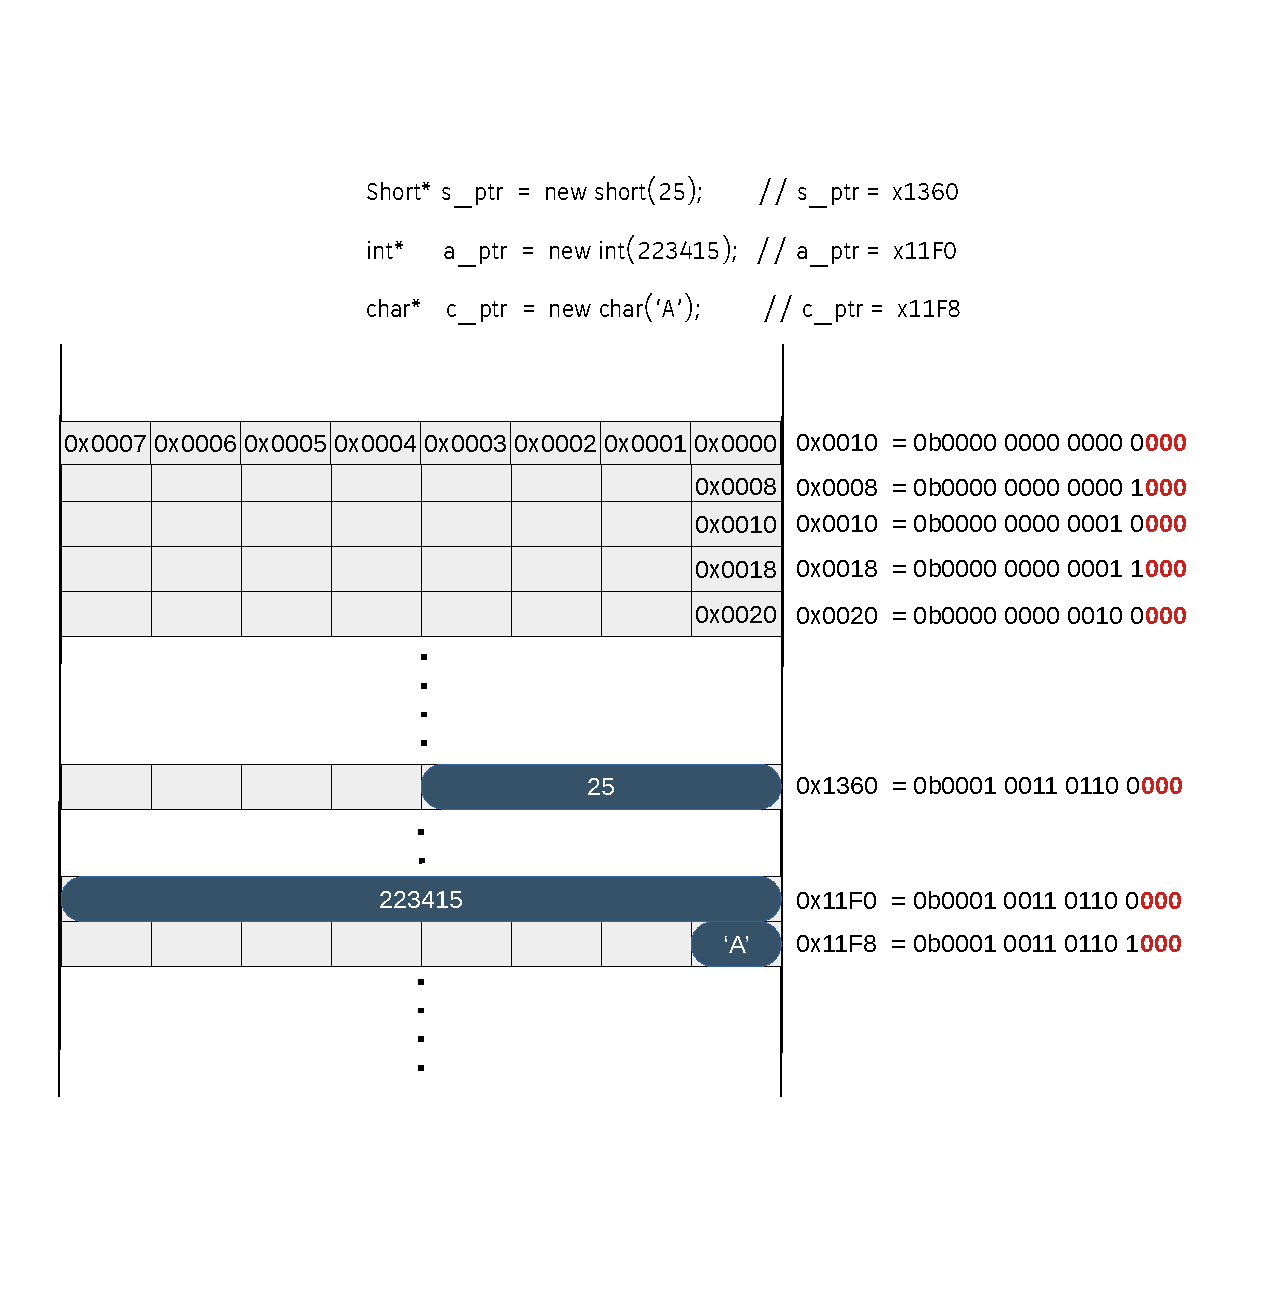
\includegraphics[scale=0.8]{figures/chapter2/memorylayout}
	\caption{An example of memory layout with data objects of various types allocated in the heap. All objects are aligned by 8 bytes so their addresses are always multiple of 8.}
	\label{fig:data_aligntment}
\end{figure}

\subsection{Tagged Pointers}
Some high-level programming languages, for example C++, offer developers a tool set to work with memory. Using such tool set, developers have access to low level memory abstraction. The main building block that enables memory management is the \textbf{pointer data type} and its ecosystem. A variable of type pointer holds a memory address of an object stored in the heap. Due to data alignment (cf. \ref{sec:data_alignment}), the memory address of any object in the heap memory is always $\alpha\cdot w$ where $w=8$ (the word size). This implies all addresses held as a pointer value are multiple of 8. A pointer thus can be 8, 16, 24, 109144, etc. But it can not be 7 or 13. \\

\begin{figure}
	\centering
	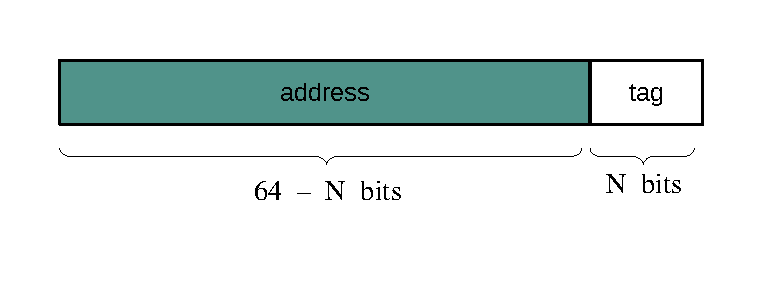
\includegraphics[scale=1]{figures/chapter2/pointervalue}
	\caption{The structure of a tagged pointer. The number of tagging bits depends on the CPU architecture. Depending on the architecture, a $ N = log_{2}(word\_size)$ of LSBs bits are dedicated for tagging. In 64-bit architecture, $word_size = 8$, thus $N = 3$.}
	\label{fig:tagged_pointer}
\end{figure}


Consequently, all pointer values share the fact that the first three low significant bits (LSBs) in their binary representation are always 0. As a result, we could exploit those bits to encode additional information without affecting the validity of the pointer (Fig. \ref{fig:tagged_pointer}).  \\ 

As a use case, depending on the tag, pointer tagging allows a dynamic representation of the numeric value held by the pointer. Thus, the actual payload of the pointer could represents a memory address for some time during the process execution but can later express the binary representation of a \texttt{char} value for example, depending on the execution context and after a change in the tag value during run-time. \\

\subsection{Tagged Pointer Implementation}

An approach to implement a tagged pointer is to develop a wrapper object around a pointer type variable. By that, we insure safety by presenting a single point of failure in case of pointer value misuse. The wrapper can be equipped with adequate behaviours that govern the tag/ payload manipulation and retrieval. \\

Accessing the binary representation of pointer to enable pointer tagging is straightforward in most programming languages and is done by using bit-wise operations. \\


\clearpage
\section{Semantic Web}
\label{sec:preliminaries:semanticweb}

Today World Wide Web (WWW) holds a tremendous amount of different types of data (videos, images, text, geolocation data, books, publications, etc.). 
Such data comes from different sources (web applications, warehouse systems, GPS devices, smartphones, ATMs, etc.).
However, such data are still processed passively by computer system as there is no way to understand its meaning or context.
The term \textbf{Semantic Web} was coined by Tim Berners-Lee for a \textit{Web of Data} (or \textit{Data Web}) \cite{LeeWeavingTheWeb} that can be processed by machines. 
The key technologies of Semantic Web are published by the World Wide Web Consortium (W3C). 
The Resource Description Framework (RDF), a standard for representing data in the Semantic Web, and SPARQL, a query language for RDF data, are introduced in this section.

\subsection{Resource Description Framework}

The Resource Description Framework (RDF) is part of the W3C standard to define the web of data \cite{rdfonline}. Regardless of the nature of the data entity held on the web (blog post, image, publication, newspaper article,  list of invoices, etc.), RDF identifies them uniformly as resources. In the standard, each resource is attached to a unique Internationalized Resource Identifier (IRI). IRI is a standard defined by the Internet Engineering Task Force in RFC 3987 \cite{Pasd}\todo{cite}. Literals are another sort of resources. A literal comprises a hardcoded value represented as a string; (“Martin,” “true”, “12.3”) are examples of literals. The third resource type is called a blank node. Blank nodes represent anonymous resources and always have local scope where they can be assigned a unique identifier. All definitions in this section are taken from “RDF 1.1 Concepts and Abstract Syntax” \cite{asd}.\todo{cite} \\

\begin{definition}[RDF Terms]
Let $I$ be the set of \textit{IRIs}, $L$ be the set of \textit{literals} and be $B$ the set of
\textit{blank nodes}. Further $I$, $L$ and $B$ are finite and pair-wise disjoint. Then the set $RT = I \cup L \cup B$ is called the set of RDF terms. 
\end{definition}

\subsubsection{RDF Triple, RDF Graph} On an abstract level, an RDF triple can be seen as a statement that describes the relationship between two resources. An RDF triple can also serve to describe the property of a resource. RDF triple is represented by a sentence composed of three elements in order: \textit{a subject}, \textit{a predicate} and \textit{an object}.
The subject is a RDF resource. The subject has a property defined by the predicate and a value for that property set by the object.
RDF restricts which RDF terms can be used for subject, predicate and object:

\begin{definition}[RDF Triple, RDF Graph]
An RDF Triple is a triple $(s, p, o) \in ( I \cup B ) \times I \times RT$ where $s$ is called subject, $p$ is called predicate and $o$ is called object. \\
A set of of RDF Triples is called RDF graph.
\end{definition}

\paragraph{Example 2.1}
An example of an RDF graph is given in Table \ref{tab:rdf_graph_example}. 
The data describes a unicorn named “Ralf ” and a lama named “Sara”. Additionally, it states that unicorns eat rainbows and lamas eat plants. \\

We use a special language to retrieve data from an RDF graph called SPARQL. SPARQL \cite{asd} is a recursive acronym for “SPARQL Protocol And RDF Query Language”. 
Listing \ref{lst:sparqlexample} shows a simple example of a SPARQL query
against the RDF graph in table \ref{tab:rdf_graph_example}. \\



\begin{table}[h]
	\centering
	\begin{tabular}{lll}
		\textbf{subject} & \textbf{predicate} & \textbf{object} \\ \hline
		ex:ralf          &        foaf:name            &          "Ralf"       \\
		ex:ralf          &        rdf:type           &       dbr:Unicorn          \\
		ex:sara			&          foaf:name          &          "Sara"       \\
		ex:sara         &            rdf:type        &           dbr:Llama   \\  
		dbr:Unicorn         &           ex:eats        &           dbr:Rainbow   \\  
		dbr:Llama      &            ex:eats      &          dbr:Plant  \\
	\end{tabular}
	\caption{An RDF graph about a lama and a unicorn, what are their names and what they eat.}
	\label{tab:rdf_graph_example}
\end{table}

\begin{lstlisting}[label={lst:sparqlexample},caption={An SPARQL query that returns what food Ralph eats.}]
SELECT ?food
WHERE { 
	?being foaf:name "Ralf" .
	?being rdf:type ?type .
	?type ex:eats ?food }
\end{lstlisting}
 
\clearpage
\section{Tentris}
\label{sec:preliminaries:tentris}

There is no standard design guideline for triple stores. Hence different implementations of triple stores co-exist. Each subgroup of these implementations utilizes a category of underlying data structures as well as corresponding algorithms that govern the behavior. 
In production, triple stores are used to store up to billions of RDF triples. 
To that extent, quality factors like efficiency and scalability are considered first-class citizens during triple stores' construction. 
And the selection of internal data structures and the behavior definitions greatly influence the overall system efficiency. \\

Fuseki, Blazegraph, Virtuoso, and RDF-3X are popular implementations of Triple stores. 
One of the key design characteristics those triple stores have in common is that they all utilize B+ trees to store the indices. 
Other categories of triple stores use 3D Boolean tensors to store and process RDF data. In such systems, each tensor dimension is mapped to a triple data aspect, i.e., subject, predicate, or object. Examples of tensor-based triple stores include systems like TensorRDF and BitMat. In the following, a novel tensor-based RDF triple store is presented. \\

Tentris is a triple store variant designed by the data science research group at Paderborn university\cite{tentris2020}. 
Tentris is an in-memory storage solution that represents RDF knowledge graphs as sparse order-3 tensors using a novel data structure, called Hypertire. 
It then uses tensor algebra to carry out SPARQL queries by mapping SPARQL operations to Einstein summation\cite{einstein}. 
At the time of this writing, Tentris' SPARQL engine realizes \textit{SPARQL-BGB}  (a subset of the SPARQL-algebra). 
Consequently, the engine can execute SPARQL queries containing the following keywords: \verb|@prefix|, \verb|SELECT|, \verb|WHERE|, and \verb|DISTINCT|\cite{foundationofthesemanticweb}. \myworries{mention that you omit talking about the query aspects: Einstein summation, etc} \\

Since my work represents a further contribution to the project Tentris, I dedicate this section to deliver a preface for the relevant aspects. In subsection \ref{sec:tensor_algebra}, I specify what tensors are. A way of representing RDF graphs in tensors is showed in subsection \ref{sec:rdf_tensor}. Hypertrie data structure is visited in subsection \ref{sec:hypertrie}.

\subsection{Tensor Algebra}
\label{sec:tensor_algebra}
In mathematics, the term Tensor holds a representation-independent meaning. According to \cite{kj}, Tensors are “objects with many indices that transform in a specific way under a change of
Basis”. This mathematical construct has many applications in physics, artificial intelligence, and other fields. However, for tensors to be applied in a practical context, a more concrete definition should be selected. Among other choices, multi-dimensional arrays are widely used as a representation for tensors. Throughout this work, a finite $n$-dimensional array for tensor representation is adopted.
Tensor was defined formally in \cite{tentris2020} as the following:

\begin{definition}[Tensor]
A mapping\\
\centerline{$T: \textbf{K} \to V$}\\
from a multi-index $\textbf{K}$ to a codomain $V$ is called tensor. $\textbf{K}$ is called \textit{key basis} of dimension $n \in \mathbb{N}$ with \\
\centerline{ $\textbf{K} = K_0 \times K_1 \times ... \times K_{n-1}, K_i \subset \mathbb{N}$ } \\
The tuple $\textbf{k} \in \textbf{K}$ is called \textit{key}, $K_i$ is called a \textit{key part basis} and $k \in K_i$ is called \textit{key part}.\\
The dimension of the key basis is also called dimension of the tensor and is denoted by ndim($T$)=$n$. Further, nnz($T$) = $|\{\textbf{k} \in \textbf{K} | T(\textbf{k})  \neq 0\}|$ denotes the \textit{ number of non-zero entries}.
\end{definition} 

To resolve a value of a tensor, we use the array subscript notation $T[k_0, .. , k_{n-1}]$. Moreover, the symbol $V^{\textbf{K}}$ denotes the set of all mappings $T: \textbf{K} \to V$. My work exclusively consider tensors $T$ with $\mathbb{B}$ or $\mathbb{N}$ as codomain and only use multi-indexes $K_1 = ... = K_n \subset \mathbb{N}$. An $n$-dimensional tensor is also called \textit{order-$n$} tensor.
\begin{example}
\label{tensors_examples}
 In the following, some examples to illustrate the Definition 2.3:

\begin{enumerate}
	\item A tensor $S \in \mathbb{Z}^{\emptyset}$ is called a \textit{scalar}.\\
	\centerline{$S = 1$}
	So $S[\emptyset] = S[]$ is 1.
	\item A tensor $X \in \mathbb{Z}^{\mathbb{N}_3}$ is called a \textit{vector}.\\
	\centerline{$X =\left[ \begin{array}{c}
		4 \\ 7 \\ 15\\
		\end{array}\right]$}\\
	where $X[2]$ is 15. 
	\item Now, we take a three dimensional tensor $Y \in \mathbb{Z}^{\mathbb{N}_2 \times \mathbb{N}_2 \times \mathbb{N}_2}$. It can be visualized by a vector for the first key part which, in turn, has matrices each with dimensions corresponding to second and third key parts. As an example:\\
	\centerline{$Y = \left[ 
		\begin{array}{c}
		\left[\begin{array}{cc}  1 & 2 \\ 3 & 5 \\\end{array} \right]\\ 
		\left[\begin{array}{cc} 7 & 11 \\ 13 & 15 \\\end{array} \right]\\ 
		\end{array}
		\right]$}\\
	Such that, $Y[1, 0, 1]$ is 11.
\end{enumerate}
\end{example}

\subsubsection{Tensor Operations}
\label{sec:tensor_operations}
This section highlights the core operations on tensors. In particular, I describe what tensor slicing and Einstein summations are. In the following, I skip the formal definitions of the operations, instead I present them informally with examples.


\paragraph{Slices} Slicing is a useful operation to retrieve a well-defined portion of a tensor $T \in V^{K}$ in the form of a lower order tensor. Slicing is done by using a \textit{slice key} $\textbf{s} \in S = (K_0 \cup \{:\}) \times .... \times ( K_{n-1}\cup \{:\})$, and denoted like as we are retrieving a value but with one or more dimensions not bound, e.g. $T[:, x, :]$ (or $T[<:, x, :>]$). 
When applying the slice key $\textbf{s}$ to a tensor $T$, the unbounded dimensions in the slice key (the ones that are marked with $:$) are kept. 
A slice key part $s_i \neq :$ removes
all entries with other key parts at position $i$ and removes $K_i$ from the resultant tensor domain. e.g., $T[:, 2, :]$ or $T[<:, 2, :>]$.

\begin{example}
	Back to the third item in Example \ref{tensors_examples}, slicing tensor $Y$ by slice keys $s_1 = <:, 1, :>$ results in an order-2 tensor $Z_1 = Y[:, 1, :]$, and with a slice key $s_2 = <0, 1, :>$ results in an order-1 tensor $Z_2 = Y[0, 1, :]$:\\
	
	 \centerline{$Z_1 = \left[ \begin{array}{cc} 1 & 2 \\ 7 & 11 \\ \end{array}\right]$}  
	 
	 
	 \centerline{$Z_2 = \left[ \begin{array}{c} 1 \\ 2 \\ \end{array}\right]$} 
\end{example}

Worth to mention that, slicing operation is associative, meaning that applying a sequence of slicing operations with different grouping to tensor $Y$ brings the same results:

\centerline{$Y[1, 0, :] = (Y[1, :, :])[0, :] = Y([:, 0, :])[1, :] = Z_2$}

\paragraph{Einstein Summation}
\label{einstein_summation}
\myworries{Need to be added}

\subsection{Storing RDF Graphs in Tensors}
\label{sec:rdf_tensor}
Based on \cite{tentris2020}, let $g$ be an RDF graph with IRIs ($I$), blank nodes ($B$) and literals ($L$) being finite sets, and thus the set of RDF terms $RT$ is also finite (Sec. \ref{sec:rdf}). We define a bijective function $id_{RT}: RT \to N_n$ where $|RT|=n$. We call the function \textit{index of resources}. $id_{RT}$ maps each RDF term to a unique identifier. Similarly, we define the \textit{resources by indices} function as $res_{RT} = id_{RT}^{-1}$. 
We omit the use of the subscript $RT$ with the functions' names $id_{RT}$ and $res_{RT}$ when it is clear from the context. \\

Every triple $<s, p, o> \in g$ is also in ($RT \times RT \times RT$). For that, we can define an order-3 tensor $T \in \mathbb{B}^{N_n \times N_n \times N_n}$. We store the triple $<s, p, o>$ in $T$ by setting $T[id(s), id(p), id(o)] = 1$ and all other entries in $T$ are set to 0. We call $T$ the tensor representation of the RDF graph g and denoted by $T_g$. In other words: \\
\centerline{$T[i_s, i_p, i_o] = 1 \iff <res(i_s), res(i_p), res(i_o)> \in g$}

\begin{example}
Figure \ref{fig:rdf_tensor} shows a 3D visualization of 3-dimensional tensor that represents the RDF graph $g$ depicted in table \ref{tab:rdf_tensor}. We notice that the number of distinct RDF terms in $g$ is 7, so we can represent $g$ with a tensor $T_g \in \mathbb{B}^{N_7 \times N_7 \times N_7}$. 
\end{example}

Since $T_g$ has the codomain $\mathbb{B}$, we describe $T_g$ as a \textit{boolean tensor}. Subject, predicate, and object are associated with one dimension each. In practice, a dimension range  ($|RT| =n$) of an RDF tensor $T_g$ fits much more than the bounded resources' IDs in $g$ for that dimension. In \cite{tentris2020}, however, it is proven that by choosing equal key part basis for enable efficient dimension matching using Einstein notation. As $T_g$ can store a super set of RDF triple in $g$, we call $T_g$ \textit{a sparse tensor}

\begin{table}[h]
	\centering
	\begin{tabular}{lll}
		\textbf{subject} & \textbf{predicate} & \textbf{object} \\ \hline
		:e1 (1) & foaf:knows (2) & :e2 (3) \\
		:e1 (1) & foaf:knows (2) & :e3 (4) \\
		:e2 (3) & foaf:knows (2) & :e3 (4) \\
		:e2 (3) & foaf:knows (2) & :e4 (5)  \\
		:e3 (4) & foaf:knows (2) & :e2 (3) \\ 
		:e3 (4) & foaf:knows (2) & :e4 (5) \\
		:e2 (3) & rdf:type (6) & dbr:Unicorn (7) \\
		:e4 (5) & rdf:type (6) & dbr:Unicorn (7) \\
	\end{tabular}
	\caption{An RDF graph example. Resources are printed alogn with their corresponding IDs (enclosed in brackets).}. 
	\label{tab:rdf_tensor}
\end{table}

\begin{figure}[h]
	\centering
	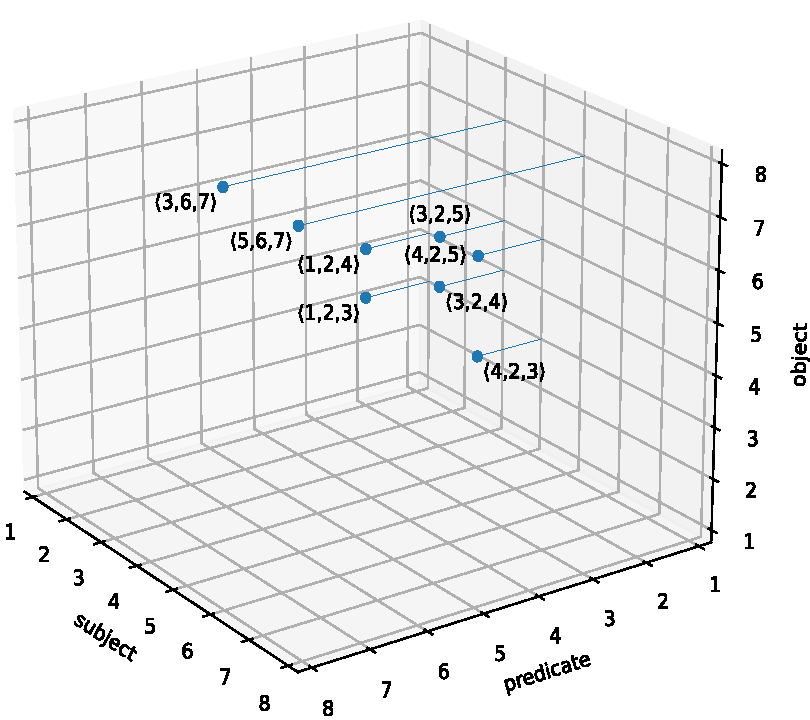
\includegraphics{figures/chapter2/3Dcoord-cut}
	\caption{A 3D plot of an order-3 RDF tensor representing the RDF graph in table \ref{tab:rdf_tensor}.}
	\label{fig:rdf_tensor}
\end{figure}

\subsection{Tentris and Hypertrie}
\label{sec:hypertrie}